\documentclass[onecolumn,12pt]{asme2ej}
\usepackage{epsfig}\usepackage{amsmath}\usepackage{amsfonts}
\usepackage{amssymb}\usepackage{graphicx}\pagenumbering{arabic}
\usepackage{verbatim}\usepackage[utf8]{inputenc}\usepackage[portuguese]{babel}
\providecommand{\keywords}[1]{\small\textbf{\textit{Keywords---}} #1}
\usepackage{comment}
\usepackage[backend=biber,style=numeric,sorting=none]{biblatex}
\usepackage{fancyhdr}
\pagestyle{fancy}\fancyhf{}\rfoot{Página \thepage}
\addbibresource{mybib.bib}\title{Conhecimentos sobre o Estado da Arte da Inteligência Artificial} \author{Gustavo Hammerschmidt\affiliation{PUCPR - Pontíficia Universidade Católica Paraná\\Ciência da Computação\\Email: g.hammerschmidt@pucpr.edu.br}}\author{João Vitor Andrioli de Souza 
\affiliation{PUCPR - Pontíficia Universidade Católica Paraná\\Ciência da Computação\\Email: joao.vitor.andrioli@pucpr.edu.br}}

\begin{document}

\maketitle

\begin{abstract} \iffalse To Do \fi
{\it 

Com a crescente importância e efeitos da imersão da Inteligência Artificial, é fundamental difundirmos o conhecimento básico e médio acerca do tópico e para isso analisarmos a compreensão atual e se as pessoas superestimam o Estado da Arte da Inteligência Artificial em relação à imersão desta ou em relação à sua tangibilidade, que é, por vezes, moldada à uma visão hollywoodiana da área do individuo. Foi observado que os entrevistados estão a par da situação atual, pois possuem boa compreensão dos conhecimentos gerais e sobre a filosofia da Inteligência Artificial, porém possuem estimativas futuras que não condizem com a realidade. A pesquisa trouxe resultados satisfatórios e esperados por parte dos estudantes de exatas. Concluímos que até mesmo os profissionais mais próximos da área e estudantes, que estão mais a par do estado da arte da I.A., possuem opiniões divergentes sobre a imersão e influência desses algoritmos no dia a dia.

}
\end{abstract}
\keywords{IA, Inteligência, Artificial, Survey, Conhecimentos, Estado, Arte}

\section{Introdução} \iffalse Done \fi

A compreensão acerca da Inteligência Artificial é, por vezes, moldada à uma visão hollywoodiana da área em questão, sendo, assim, às vezes, uma visão destoante do estado da arte. Pessoas leigas no assunto, em geral, veem a Inteligência Artificial como um robô semelhante a forma humana, capaz de realizar tarefas complexas com maior eficiência às vezes do que a de ser humano; e não a veem como um algoritmo sem forma tangível, que baseia suas decisões baseando-se em padrões matemáticos ou computáveis muito mais do que em comparação ao humano - que, por vezes, chega as suas conclusões por intuição, ou simplesmente, não é capaz de provar o seu raciocínio logicamente para obtê-las ainda que estejam certas suas conclusões. Há também aqueles, imperitos no tópico, que creem não estarem em uma realidade onde a Inteligência Artificial ou algoritmos de I.A. já atuam ou auxiliam diariamente com certas atividades em suas vidas.

A crescendo utilização das técnicas de inteligencia artificial, levantou preocupações sobre os avanços e as consequências da inteligencia artificial e como afeta a vida humana, como o trabalho humano e as capacidades serão modificadas e melhoradas ou pioradas. Será que um algoritmo conseguira atingir inteligencia superior a humana?

Nossa pesquisa identificou que, contudo, até mesmo os profissionais mais próximos da área e estudantes, que estão mais a par do estado da arte da I.A., possuem opiniões divergentes sobre a imersão desses algoritmos e o que, para eles, é uma consciência ou se uma I.A. é consciente de si.

\section{Trabalhos Relacionados} \iffalse Done \fi

Estudos\cite{survey_1}\cite{survey_2} exploraram o ambiente e espaço ativo da Inteligência Artificial e os pontos de contato com o ser humano,\cite{survey_3}\cite{survey_4} a ética de uso e efeitos legais possíveis e desejáveis da Inteligência Artificial, o futuro previsto da opinião humana sobre o tópico e como será o futuro da área e os impactos nos profissionais e imperitos no assunto \cite{survey_5}\cite{survey_6}, comentando os grandes efeitos e que todos serão afetados.

Artigos também levantam os impactos e implicações especificas de profissão, como o jornalismo no contexto da digitalização e a Inteligência Artificial, onde a representação e utilização de Inteligência Artificial no mundo é tão ampla que se torna difícil discernir a realidade do estado da arte atual e o pensamento fictício dos filmes, principalmente com as ocorrências atuais dos carros autônomos, drones de entrega e algoritmos que mimicam a razão e o pensamento humano \cite{survey_7}.

\section{Método de Pesquisa} \iffalse Done \fi

Para realizar nossa pesquisa, a conduzimos no formato Survey, definindo uma enquete com as perguntas(Seção 3.1.3: Questionário) a respeito do tópico, e a enviamos aos estudantes de Ciência da Computação da PUCPR.

\subsection{Planejamento do Survey} \iffalse Done \fi
 
 Utilizamos o protocolo de Survey proposto e comentado por Freitas et al. \cite{survey_8} descrito pela obtenção de dados, informações e características de um grupo de pessoas sobre um assunto. 
 
 Nosso estudo é descritivo e de corte-transversal, pois descreve a distribuição de conhecimento e opiniões acerca da Inteligência Artificial, faz uma comparação entre as distribuições e tem como propósito verificar se a percepção dos fatos está ou não de acordo com a realidade do estado da arte no tópico, corte-transversal significa que a coleta de dados ocorre em um só momento, pois não pretendemos analisar a evoluções das opiniões.
 
 Consideramos como restrições pessoas menores de 18 anos e maiores de 35 anos, devido a falta de contato e experiencia sobre o assunto, no entanto nenhuma pessoa se enquadrou nesta restrição, a amostra alvo foi categorizada e separada pela areá de trabalho e estudo, pois isto pode afetar os resultados, dado que a área de exatas é composta por uma maior quantidade de criadores de técnicas de Inteligência Artificial.
 

\subsubsection{Caracterização da Amostra} \iffalse Done \fi

A amostra dos entrevistados tem como enfoque estudantes, professores ou profissionais de áreas sujeitas a terem um maior contato com Inteligências Artificiais. Para a coleta dos dados, a enquete fora destinada às seguintes áreas de estudo: Ciência da Computação, Engenharia, Jornalismo, Medicina e Psicologia da PUCPR. No entanto, apenas estudantes de Ciência da Computação responderam à enquete; tentamos contactar os coordenadores das outras áreas, infelizmente, sem respostas. Obtivemos 15 respostas à enquete, destas todos os estudantes responderem ser de Exatas e 93\% dos deles estão na faixa etária de 18 a 25 anos; tendo apenas um estudante na faixa de 30 e 35 anos. 

\subsubsection{Hipóteses} \iffalse Done \fi

Hipóteses foram estabelecidas para determinar se a amostra está a par do estado da arte da I.A. São elas:
$\\ \\$
- Hipótese Nula:
$\\$ As pessoas não superestimam o Estado da Arte da I.A. em relação à imersão desta ou em relação à sua tangibilidade. 

$\\$ 
- Hipótese Alternativa:
$\\$ As pessoas superestimam o Estado da Arte da I.A. em relação à imersão desta ou em relação à sua tangibilidade.

\subsubsection{Questionário} \iffalse Done \fi

Separamos o questionário em 4 grupos: Filtragem e Dados Básicos, Conhecimentos Gerais, Estimativas do Entrevistado e curiosidades. 

O grupo Filtragem e Dados Básicos fornece a idade e a área de estudo dos entrevistados; o grupo Conhecimentos Gerais fornece os dados necessários para analisar se o entrevistado possui algum conhecimento sobre tópicos específicos que são a base de diversas tarefas de Inteligências Artificiais, como estatística e redes neurais; o grupo de Estimativas do Entrevistado tem como objetivo estimular o entrevistado a pensar e opinar em alguns tópicos atuais sobre as I.A.'s, a relação da falta de trabalho com a automação que ao mesmo tempo gera trabalhos para especialistas na automação e comparações entre a inteligência artificial real e fictícia; e o grupo das Curiosidades tem como objetivo definir os limites e o nível de imaginação empregados pelos entrevistados, as perguntas são difíceis de responder pois envolvem termos complexos que são fortemente ligados ao ser humano e a conceitos com respostas que ainda divergem entre as pessoas(o ser humano é complexo). Abaixo segue o questionário com as perguntas dividas por seção e acompanhadas de suas possíveis respostas entre parênteses logo abaixo:

\begin{enumerate}

   \item Filtragem e Dados Básicos:
   \begin{itemize}
     \item[$*$] Qual a sua idade?
     \item[$-$]$\ \ $(menos de 18 anos, 18 - 25, 25 - 30, 30 - 35, mais de 35 anos.)
     \item[$*$] Qual a sua área de estudo?
     \item[$-$]$\ \ $(Exatas, Humanas, Biológicas, Outros.)
   \end{itemize}
   
   \item Conhecimentos Gerais:
   \begin{itemize}
     \item[$*$] Você conhece análise exploratória de dados?
     \item[$-$]$\ \ $(Sim, muito; Sim, um pouco; Não, mas já ouvi falar; Não, não conheço.)
     \item[$*$] Você possui conhecimento de estatística ou cálculo matemático?
     \item[$-$]$\ \ $(Sim, muito; Sim, um pouco; Não, mas já ouvi falar; Não, não conheço.)
     \item[$*$] Você tem conhecimento em Redes Neurais?
     \item[$-$]$\ \ $(Sim, muito; Sim, um pouco; Não, mas já ouvi falar; Não, não conheço.)
   \end{itemize}
    
   \item Estimativas do Entrevistado:
   \begin{itemize}
     \item[$*$] Em sua opinião, a Inteligência Artificial está mais relacionada com quais filmes abaixo:
     \item[$-$]$\ \ $(Ex Machina; Chappie; Eu, Robô; Ela, filme de Spike Jonze, 2013; Homem de Ferro - Assistente Jarvis; Homem de Ferro - Ultron; Ghost In The Shell; Tron.)
     \item[$*$] Você acha que a I.A. pode roubar seu trabalho?
     \item[$-$]$\ \ $(Sim; Não.)
     \item[$*$] Qual a sua estimativa de tempo para que I.A.s estejam imersas em nossa realidade?
     \item[$-$]$\ \ $(3 anos; 5 anos; 10 anos; 15 anos.)
     \item[$*$] Você utilizaria um táxi ou Uber sem motorista, um carro autônomo?
     \item[$-$]$\ \ $(Sim; Talvez; Não.)
   \end{itemize}
  
   \item Curiosidades:
   \begin{itemize}
     \item[$*$] Você acha que uma Inteligência Artificial pode ser consciente de si?
     \item[$-$]$\ \ $(Sim; Não.)
     \item[$*$] Você acha que uma Inteligência Artificial é capaz de sentir?
     \item[$-$]$\ \ $(Sim; Não.)
     \item[$*$] Você acredita que somos capazes de definir o que é consciência e/ou Inteligência?
     \item[$-$]$\ \ $(Sim; Não.)
     \item[$*$] Em sua opinião, o pensamento é puramente lógico?
     \item[$-$]$\ \ $ (Sim; Não.)
     \item[$*$] Uma I.A., feita para criar obras de arte, aprende a desenhar com quadros famosos, esta I.A. é original em suas obras ou uma cópia da cópia?
     \item[$-$]$\ \ $ (Original, Cópia da Cópia.)
   \end{itemize}

\end{enumerate}

\subsection{Execução do Survey} \iffalse Done \fi

Para garantir a qualidade do estudo, empregamos um teste piloto utilizando o questionário composto por 14 perguntas para os 15 participantes, efetivando a filtragem e restrições de qualidade, além de discutir com atuantes da área que ajudaram a melhorar as perguntas, tópicos e formatos.

\subsubsection{Teste Piloto} \iffalse Done \fi

Os procedimentos de aplicação da pesquisa Survey\cite{survey_8} foram feitos por meio de um documento tipo questionário do Google forms, que foi distribuído para os estudantes de Ciência da Computação durante as aulas de Métodos de Pesquisa em Computação. Os procedimentos de limpeza dos dados obtidos foram feitos do seguinte modo: primeiro, selecionamos os dados de faixa etária "menos de 18 anos" ou "mais de 35 anos"; e, por último, selecionamos os dados pertencentes a área de estudo "exatas" somente - conforme apontado nas figuras 1 e 2, respectivamente, respostas de idade e respostas de áreas de estudo.

\begin{figure}[h]
  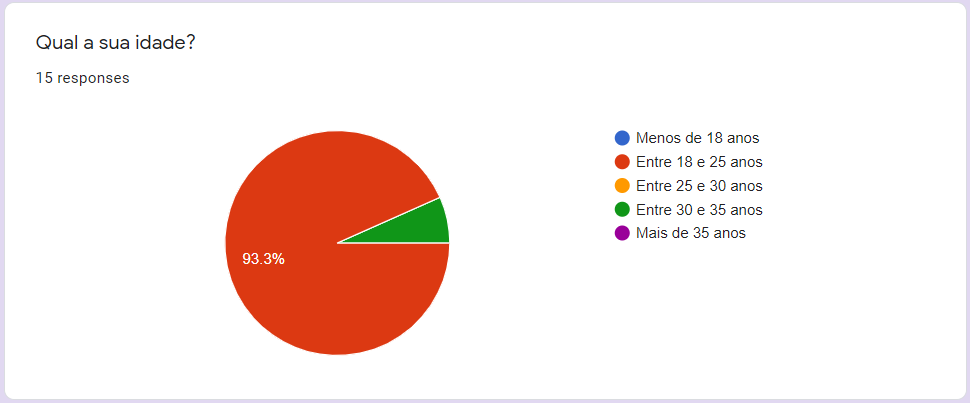
\includegraphics[width=\linewidth]{pictures/idade_pic.PNG}
  \caption{Respostas de idade}
  \label{fig:idades}
\end{figure}

\begin{figure}[h]
  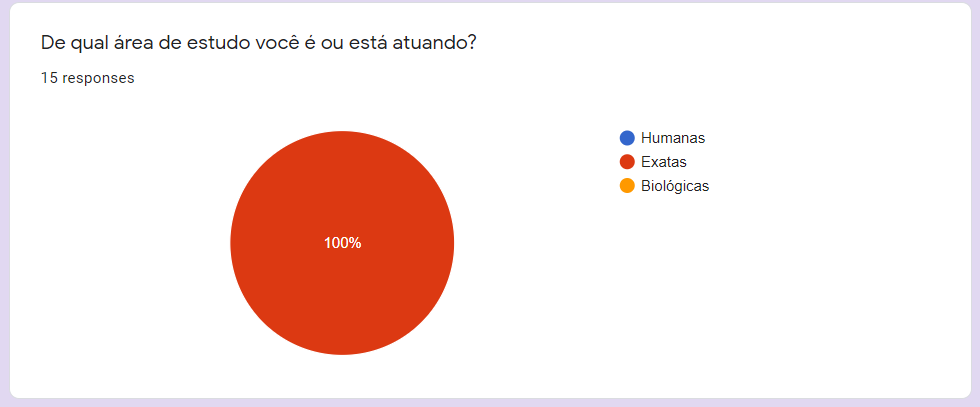
\includegraphics[width=\linewidth]{pictures/area_pic.PNG}
  \caption{Respostas de áreas de estudo}
  \label{fig:areas_de_estudo}
\end{figure}


A qualidade mensurada dos dados de forma exploratória depois das etapas de aplicação e limpeza foi satisfatória, proporcionando uma heterogeneidade nas respostas obtidas devido a complexidade das perguntas, como é possível notar nas figuras 3 e 4, respectivamente, respostas de análise exploratória e respostas de estimativa de tempo.

\begin{figure}[h]
  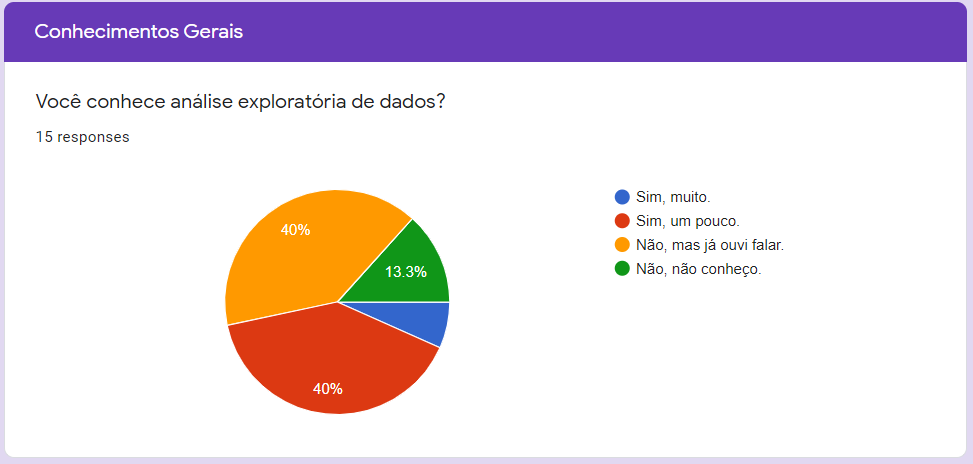
\includegraphics[width=\linewidth]{pictures/cg_pic.PNG}
  \caption{Nível de conhecimento sobre análise exploratória de dados.}
  \label{fig:analise_exploratoria}
\end{figure}

\begin{figure}[h]
  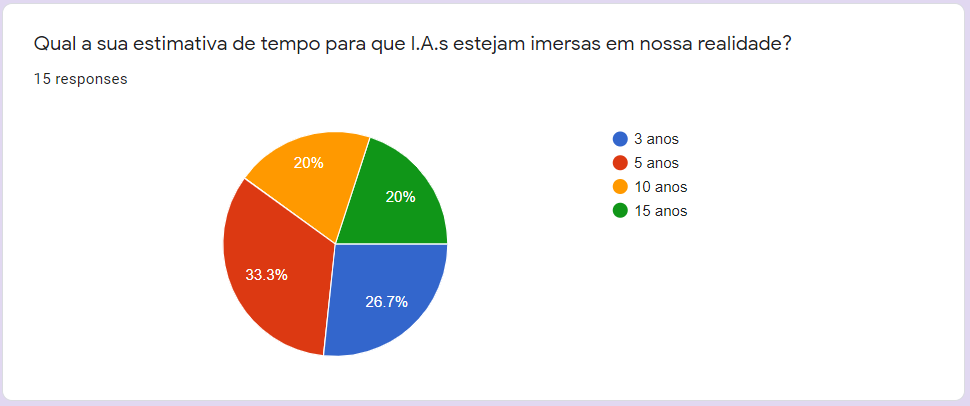
\includegraphics[width=\linewidth]{pictures/est_pic.PNG}
  \caption{Respostas de estimativa de tempo para imersão de I.A.'s}
  \label{fig:estimativa_de_tempo}
\end{figure}

\subsubsection{Distribuição do Questionário} \iffalse Done \fi

A nossa equipe distribuiu o questionário durante as aulas de métodos de pesquisa em computação via blackboard collaborate, via discord e via WhatsApp; os entrevistados foram separados em grupos conforme as figuras 1 e 2 no que tange suas faixas etárias e suas áreas de estudo respectivamente. O questionário fora feito no formato google forms.

\section{Discussão dos Resultados} \iffalse Done \fi

Nossa equipe formulou uma hipótese a respeito do conhecimento do estado da arte da Inteligência Artificial dos entrevistados e se possui uma visão deturpada do estado atual.

Para identificar se a nossa hipótese é sustentada, dividimos as respostas em seções cujas perguntas almejavam dificultar conforme a ordem da seção aumentava; sendo, assim, a seção de Conhecimentos Gerais a nossa etapa básica a respeito do tema. Nela foram identificados que: 

\begin{figure}[h]
    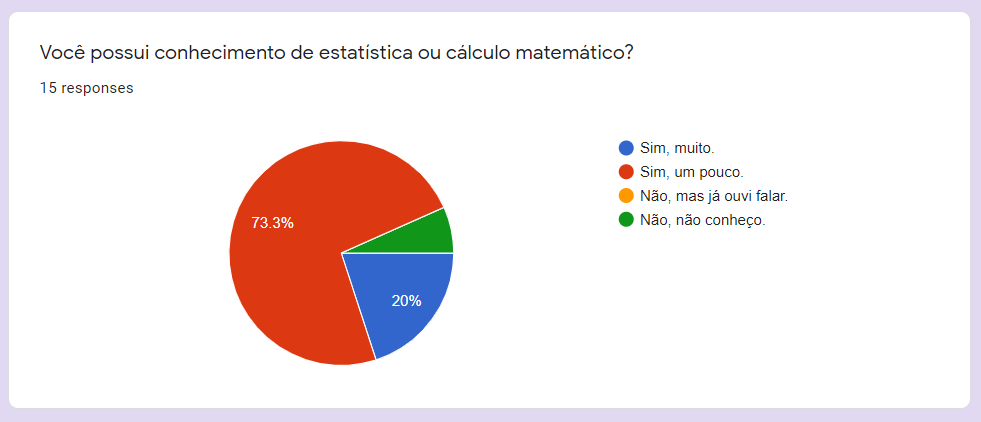
\includegraphics[width=\linewidth]{pictures/cec_pic.PNG}
    \caption{Nível de conhecimento sobre estatística e cálculo matemático.}
    \label{fig:estatistica_e_matematica}
\end{figure}

\begin{figure}[h]
    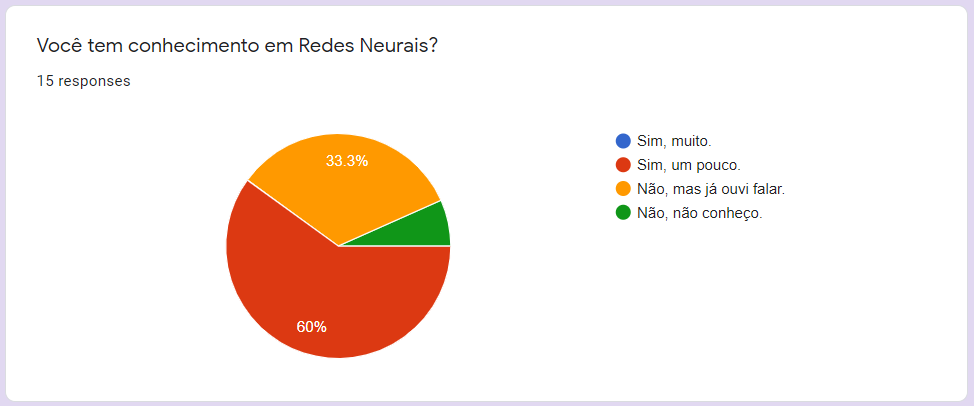
\includegraphics[width=\linewidth]{pictures/crn_pic.PNG}
    \caption{Nível de conhecimento sobre Redes Neurais.}
    \label{fig:redes_neurais}
\end{figure}


\begin{enumerate}
  \item Apenas 15\% dos entrevistados não possui conhecimento análise exploratória, que é a descoberta de padrões não-óbvios em conjuntos de informações; e que 53.3\% possuem algum conhecimento do tópico. (Já apresentada na seção 3.2.1, Figura 3.)
  \item 93.3\% dos entrevistados possuem algum conhecimento a respeito de estatística ou cálculo matemático. (Figura 5.)
  \item 60\% dos entrevistados tem conhecimento em redes neurais e 33.3\% já ouviram falar sobre o tópico. (Figura 6.)
\end{enumerate}

Os resultados apontados indicam que a maioria da amostra possui um nível de proximidade alto com os tópicos base sobre I.A.'s. 


Na seção Estatísticas, foram identificados que:

\begin{figure}[h]
    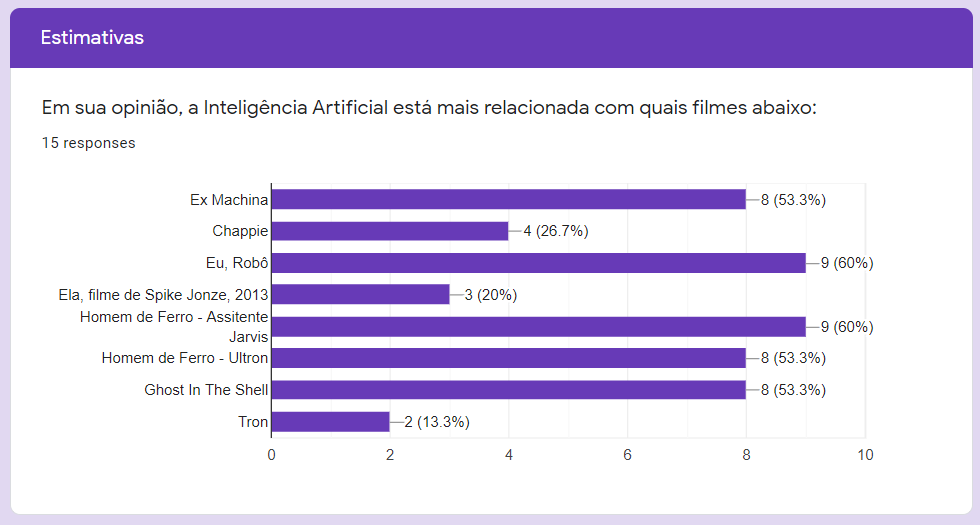
\includegraphics[width=\linewidth]{pictures/ef_pic.PNG}
    \caption{Relação da Inteligência Artificial com filmes famosos.}
    \label{fig:filmes}
\end{figure}

\begin{figure}[h]
    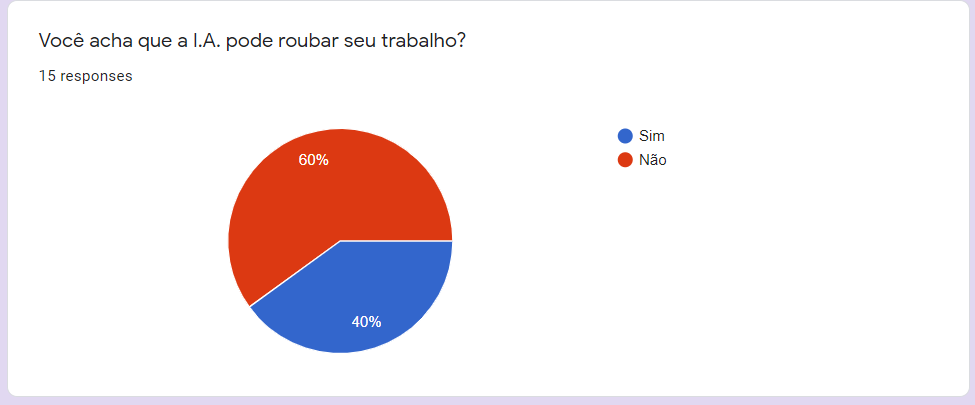
\includegraphics[width=\linewidth]{pictures/ert_pic.PNG}
    \caption{Reposta se a Inteligência Artificial pode roubar o trabalho dos participantes.}
    \label{fig:roubar_trabalho}
\end{figure}

\begin{figure}[h]
    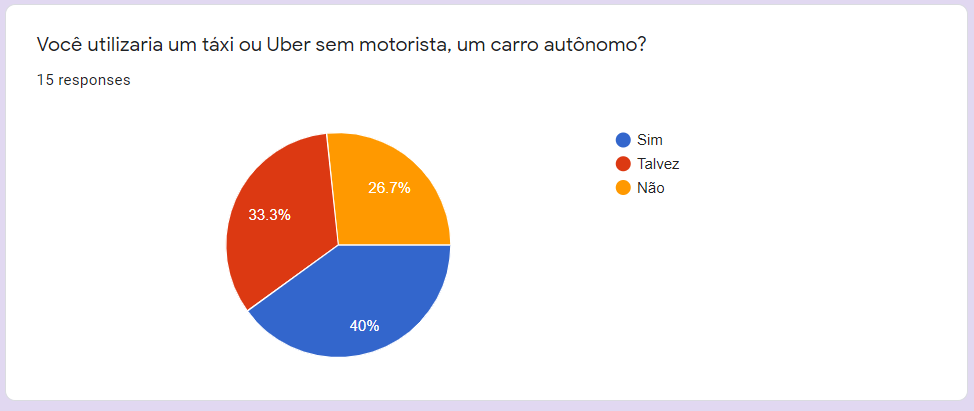
\includegraphics[width=\linewidth]{pictures/eut_pic.PNG}
    \caption{Reposta se o participante utilizaria um carro autônomo.}
    \label{fig:vermelho_carro}
\end{figure}

\begin{enumerate}
  \item Sobre a escolha dos filmes, vale ressaltar que cada entrevistado teve como opção a escolha de todos os filmes, mas deveria ao menos selecionar um. Os resultados, contudo, mostram que os Filmes Tron e Ela são os filmes menos votados e isso impacta positivamente a nossa hipótese, pois, nestes filmes as I.A.'s são intangíveis(Tron e Ela) e estão restritas a um ambiente(um jogo virtual e um aplicativo de assistente de celular respectivamente), áreas em que as I.A.'s tiveram um notável aprimoramento nas últimas décadas e são elegíveis como exemplos a representarem, hoje, o estado da arte das I.A.'s. Entretanto, as opções com mais votos estão de acordo com uma visão mais hollywoodiana do que seria uma Inteligência Artificial e não representam o estado atual. (Figura 7.)
  \item Quanto a expectativa de I.A.'s "roubarem" os seus trabalhos, 60\% dos entrevistados disse não acreditar, e esta é, à visão de nossa equipe, a opção correta a julgar pelo estado da arte, uma vez que esses algoritmos são bons ou muito bons em executar apenas uma tarefa e, portanto, não sendo exatamente "inteligentes", posto em vista que tarefas humanas demandam, geralmente, muitas competências e um grau médio ou razoável de conhecimento delas. (Figura 8.)
  \item A estimativa de tempo para que as Inteligências Artificiais estejam imersas em nossa realidade divergiu consideravelmente, com respostas variando entre 3 e 15 anos. A hipótese nula é falsa quando a grande maioria das estimativas de tempo são pequenas, preferencialmente 3 anos, pois demostra que os participantes não acreditam que a Inteligência Artificial já esta imersa em nossa realidade, o que é falso dado que atualmente nós já estamos imersos por vários algoritmos de Inteligencia Artificial, isso nega a hipótese nula e corrobora com nossa hipótese alternativa. (Já apresentada na seção 3.2.1, Figura 4.)
  \item As opiniões a respeito do uso de um carro autônomo foram divergentes e indicam apenas 40\% delegariam facilmente a atividade de dirigir a um algoritmo de Inteligência Artificial, enquanto, o restante da amostra não está tão confiante de um algoritmo desses seria capaz de garantir segurança no trânsito. (Figura 9.) 
\end{enumerate}

Os resultados apontados indicam que a maioria da amostra não está ciente, estatisticamente, da imersão desses algoritmos em algumas atividades rotineiras atualmente e que estão incertos do que exatamente identifica uma I.A.'s ou delimita suas capacidades e campo de atuação.


Na seção Curiosidades, foram identificados que:

\begin{figure}[h]
    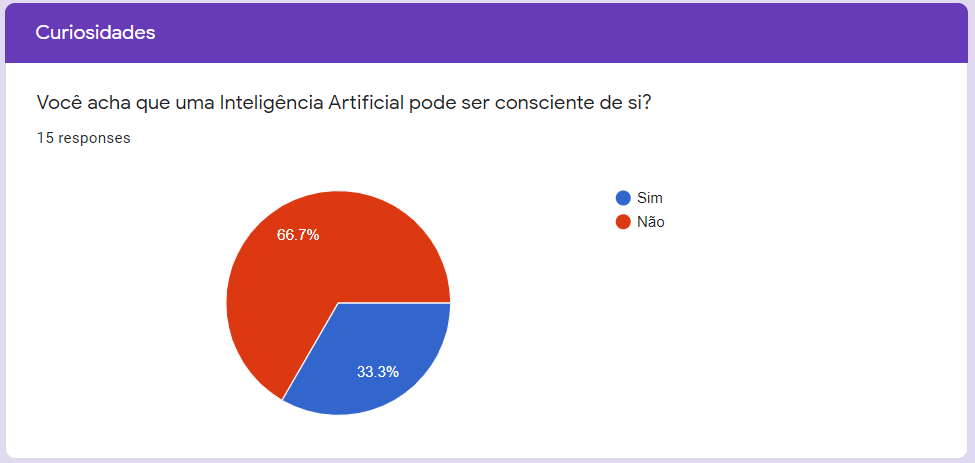
\includegraphics[width=\linewidth]{pictures/ccs_pic.PNG}
    \caption{Reposta se a Inteligência Artificial é consciente de si.}
    \label{fig:consciencia_propria}
\end{figure}

\begin{figure}[h]
    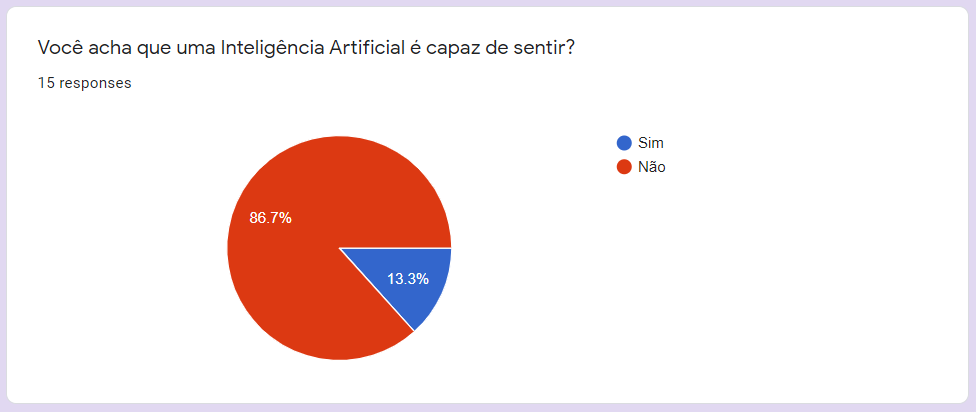
\includegraphics[width=\linewidth]{pictures/cias_pic.PNG}
    \caption{Reposta se a Inteligência Artificial é capaz de sentir.}
    \label{fig:sentimento}
\end{figure}

\begin{figure}[h]
    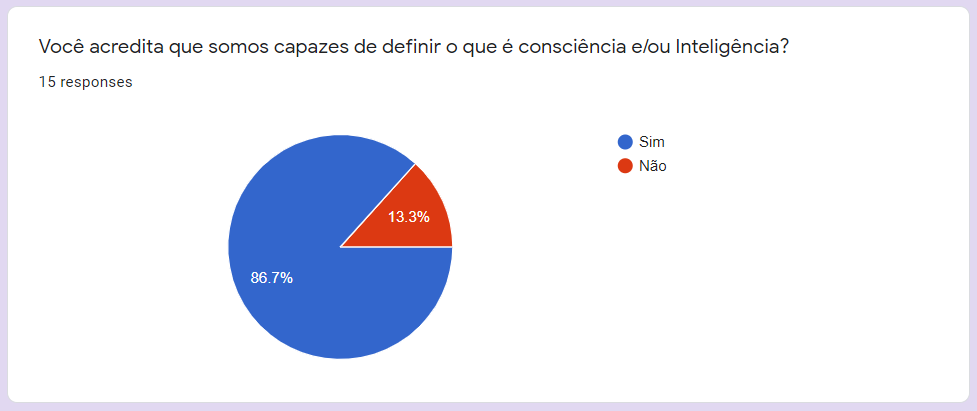
\includegraphics[width=\linewidth]{pictures/cdc_pic.PNG}
    \caption{Reposta se somos capazes de definir consciência e/ou Inteligência.}
    \label{fig:consciencia_inteligencia}
\end{figure}

\begin{figure}[h]
    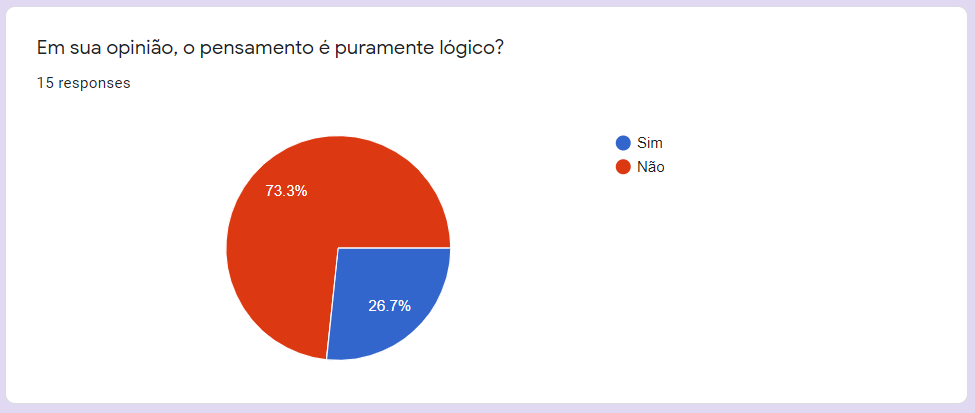
\includegraphics[width=\linewidth]{pictures/cpl_pic.PNG}
    \caption{Reposta se o pensamento é puramente lógico.}
    \label{fig:pensamento_logico}
\end{figure}

\begin{figure}[h]
    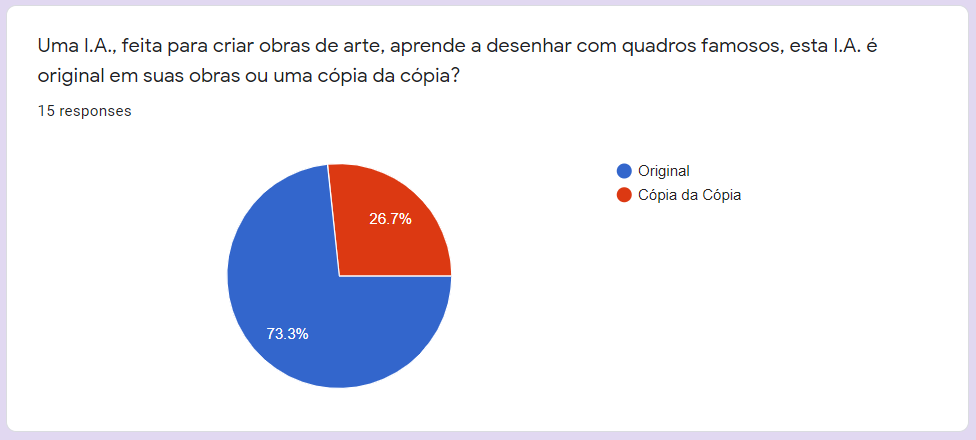
\includegraphics[width=\linewidth]{pictures/cfcoa_pic.PNG}
    \caption{Reposta acerca da originalidade artística da Inteligência Artificial.}
    \label{fig:arte_original}
\end{figure}

\begin{enumerate}
  \item A opinião da maioria está de acordo com a nossa opinião a respeito do estado da arte e do que nós consideramos ser uma limitação, pois, para nós, nem mesmo os humanos são capazes de serem totalmente conscientes de si; já que muito do que observamos e agimos sobre, diariamente, se limita ao subconsciente e não possui, para todos os casos, necessariamente, um motivo lógico para a escolha de determinado comportamento. Logo, uma Inteligência Artificial, que, segundo o estado da arte, não é de todo "inteligente" -- pois esta se restringe na maioria dos casos observados a execução com acurácia de uma tarefa apenas, não é, pelo menos atualmente, consciente de si. (Figura 10.)
  \item As maquinas não possuem a capacidade de ter sentimentos humanos, entretanto possuem a capacidade de mimetizar essas reações humanas, o que passa a falsa sensação de da vivencia de emoções. Primeiramente a Inteligência Artificial reage a estímulos de forma ostensiva e sistemática, sendo algo esperado e com um objetivo em mente. As emoções afetam e são afetadas por questões reais de forma que podemos relacionar objetos reais com a emoção sendo este o meio de funcionamento e viabilidade de mimetização da emoção pelas maquinas, as emoções humanas também estão ligadas com questões sociais, influenciadas pela época e local. 86\% dos entrevistados votou que a Inteligência Artificial não é capaz de sentir, isso corrobora com a hipótese nula. (Figura 11.)
  \item 86\% dos entrevistados acreditam que somos capazes de definir o que é consciência e/ou inteligência, isso nega a hipótese nula, pois a definição de consciência e/ou inteligência ainda é um tema discutido e que até o momento possui tópicos sem resposta. E, segundo a nossa opinião, uma função complexa, que possibilite a I.A. de ser consciente a respeito de outras partes de seu código, não conseguiria explicar porque ela pensa da forma como pensa, logo sendo incapaz de descrever a si mesmo. (Figura 12.) 
  \item  A opinião de 73.3\% dos entrevistados vai ao encontro da nossa opinião, pois acreditamos que muitas coisas no pensamento humano são difíceis de serem explicitadas de forma lógica, como sentimentos ou sonhos até mesmo; logo, quando perguntamos se o pensamento de uma I.A. pode estar completo sendo apenas lógico, queremos saber se os entrevistados julgam apenas isso como definição de pensamento ou se este é algo além disto. (Figura 13.)
  \item  Quando formulamos a pergunta, a equipe achou que sua resposta era um tanto óbvia; contudo, 73.3\% dos entrevistados afirmaram que esta I.A. seria original em suas obras, mas a nossa opinião é de que uma I.A. é treinada usando modelos ou dados de referência, logo, uma I.A. que desenha basearia-se nas técnicas de outros pintores e também suas ideias de como fazer, pois, para esta I.A. não falta técnica, falta inspiração: a parte pouco lógica ou irracional do cérebro humano. Portanto, uma I.A. dessas poderia pintar como Leonardo Da Vinci, mas dificilmente seria o próximo Da Vinci. (Figura 14.)
\end{enumerate}

Os resultados apontados indicam que 3 de 5 questões foram respondidas de acordo com aquilo que a equipe esperava como resposta, logo, confirmando que, pelo menos, a respeito de curiosidades, a maioria dos entrevistados tem boa noção do estado da arte da I.A. e aquilo que é fictício ou uma visão hollywoodiana.

Para a equipe, a amostra esteve de acordo com as nossas ideias nas seções Conhecimentos Gerais e Curiosidades, estando com um desempenho médio apenas na seção Estatísticas. Com os resultados obtidos, a equipe concluiu que a amostra valida a hipótese nula, então os estudantes de exatas entrevistados não superestimam o estado da arte da I.A. em relação à imersão desta em nossas vidas ou em relação à sua tangibilidade.

\section{Ameaças à validade} \iffalse Done \fi

Foram ameaças à nossa pesquisa, a quantidade pequena de respostas ao questionário e a pequena heterogeneidade nos dados obtidos referentes à área de estudo, limitando a nossa hipótese à área de exatas.

\section{Conclusão} \iffalse Done \fi

Neste estudo, concluímos que os estudantes de exatas entrevistados, não superestimam o estado da arte da Inteligência Artificial em relação à imersão desta em nossas vidas ou em relação à sua tangibilidade; tendo a maioria dos estudantes respondido às seções de conhecimentos gerais e curiosidades de acordo com aquilo esperado por nossa equipe. A compreensão acerca da Inteligência Artificial é, por vezes, moldada à uma visão hollywoodiana da área em questão, sendo, assim, às vezes, uma visão destoante do estado da arte. Nossa pesquisa identificou que até mesmo os profissionais mais próximos da área e estudantes, que estão mais a par do estado da arte da I.A., possuem opiniões divergentes sobre a imersão desses algoritmos e o que, para eles, é uma consciência ou se uma I.A. é consciente de si. 

Nossa equipe entende que, por vezes, a representação e inserção das I.A.'s no dia a dia é ampla e difícil de discernir entre o seu estado da arte do que é apenas ficção a seu respeito; pois, cada vez mais, ela está inserida em nossas rotinas como o uso de carros autônomos, drones de entrega ou algoritmos que mimicam a razão e o pensamento humano. O trabalho contribuiu com uma analise transitiva de corte-transversal, demostrando o conhecimento geral das pessoas de exatas sobre o estado da arte da Inteligência Artificial, que influencia o avanço e a qualidade futura dos algoritmos.


\iffalse Done \fi
\printbibliography

\end{document}
